

\rule{\textwidth}{0.4pt} 
\class{ExpertViewFilter}
public class ExpertViewFilter implements NavbarElement 

\begin{minipage}{0.3\textwidth}
    \begin{figure}[H]
        \includegraphics[scale = 0.6]{media/frontend/view/de.view.elements.navbar/ExpertviewFilterClass.png}
    \end{figure}
    \end{minipage} \hfill
    \begin{minipage}{0.6\textwidth}
ExpertViewFilter ist eine Erweiterung für erfahrene Benutzer, welche bei Aktivierung in der Navigationsbar auswählen können welche Sensortypen sie angezeigt haben wollen. Die Klasse implementiert das Interface NavbarElement, mit welchem die Funktion in der Navigationbar angezeigt wird.
\end{minipage}

Methoden:
\begin{itemize} 
    \item \emph{public void show()} Zeigt die Möglichkeit in der Toolbar an in welcher man den Experten Modus an beziehungsweise ausmachen kann. Bei Aktivierung des Moduses aktualisiert sich die Navigationsbar und fügt die Funktion hinzu mit welcher spezifische Sensortypen gewählt werden können.
    \item \emph{public void setSelectedSensors(ArrayList<Sensor> selectedSensorTypes)} Setzt die von dem Benutzer ausgewählten Sensoren
    \item \emph{public ArrayList<Sensor> getSelectedSensors()} Gibt die ausgewählten Sensoren als ArrayList weiter.
\end{itemize}

\rule{\textwidth}{0.4pt} 
\class{Navbar}
public class Navbar implements ObservedNavbarSubject, NavbarElement

\begin{minipage}{0.3\textwidth}
    \begin{figure}[H]
        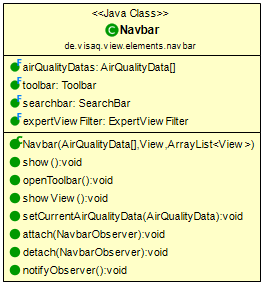
\includegraphics[scale = 0.5]{media/frontend/view/de.view.elements.navbar/NavbarClass.png}
    \end{figure}
    \end{minipage} \hfill
    \begin{minipage}{0.6\textwidth}
Die Navbar zeigt die Navigationsbar und erlaubt es dem Benutzer auf die Hilfe, Suchleiste, Sprache, Toolbar und die Luftqualitätsfilter zuzugreifen.  Die Klasse implementiert das Interface NavbarElement, mit welchem die Funktion in der Navigationbar angezeigt wird.  Es handelt sich hierbei um ein Element aus dem Beobachter Entwurfsmuster.
\end{minipage}

Attribute:
\begin{itemize} 
    \item \emph{public final AirQualityData[] airQualityDatas} Die vier auf der Webapplikation angezeigten Luftqualitätsdaten werden hier gespeichert um leichter angezeigt werden zu können
    \item \emph{public final Toolbar toolbar} Die Toolbar, welche durch den Benutzer geöffnet werden kann.
    \item \emph{public final SearchBar searchbar} Die Suchleiste in welche der Benutzer entweder Stadt, oder Postleitzahlen eingeben kann und somit die KArte an die richtige Stelle heranzoomt.
    \item \emph{public final ExpertViewFilter expertViewFilter} Der Experten Modus, welcher in der Navbar erweiterte Funktionen hinzufügt
    
\end{itemize}
Methoden:
\begin{itemize} 
    \item \emph{public Navbar(AirQualityData[] airQualityDatas, InformationView informationView, Toolbar toolbar, SearchBar searchbar, ArrayList<View> views)} Konstruktor für eine neue Navigationsbar
    \item \emph{public void show()} Zeigt die Suchleiste
    \item \emph{public void showView()} Aktiviert die aktuelle View
    \item \emph{public void openToolbar()} Zeigt die Toolbar sobald der Benutzer über die Navbar fährt und schließt sich wenn der Benutzer die Navbar oder Toolbar mit seiner Maus verlässt. 
    \item \emph{public boolean showAirQualityDatas} Zeigt die verfügbaren Luftqualitätsdata als Knöpfe in der Navbar über welche die Luftqualitätsdata Overlays gewechselt werden können.
    \item \emph{public void setCurrentView(View view)} Setzt die aktuelle View
    \item \emph{public void setCurrentAirQualityData(AirQualityData currentAirQualityData)} Setzt die aktuelle Luftqualitätsdata
    \item \emph{public void attach(NavbarObserver navbarObserver)} Erstellt eine Verbindung aus der Liste der Observer, zwischen dem Observer und Subjekt her
    \item \emph{public void detach(NavbarObserver navbarObserver)} Entfernt die Verbindung aus der Liste der Observer, zwischen dem Observer und Subjekt
    \item \emph{public void notifyObserver()} Gibt dem Observer weiter was in der Navigationbar passiert, wodurch die Suchleiste und die Karte aktualisiert wird.
\end{itemize}

\rule{\textwidth}{0.4pt} 
\class{SearchBar}
public class SearchBar implements NavbarElement.

\begin{minipage}{0.3\textwidth}
    \begin{figure}[H]
        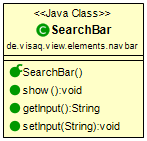
\includegraphics[scale = 0.6]{media/frontend/view/de.view.elements.navbar/SearchbarClass.png}
    \end{figure}
    \end{minipage} \hfill
    \begin{minipage}{0.6\textwidth}
Suchleiste die der Benutzer benutzen kann um nach bestimmten Städten oder Postleitzahlen zu suchen. Die Klasse implementiert das Interface NavbarElement, mit welchem die Funktion in der Navigationbar angezeigt wird.
\end{minipage}

Methoden:
\begin{itemize} 
    \item \emph{public Seachbar()} Konstruktor für die Suchleiste.
    \item \emph{public void show()} Zeigt die Suchleiste in der Navigationsbar.
    \item \emph{public String getInput()} Gibt den Benutzer input weiter und erlaubt die weitere Benutzung dieser.
    \item \emph{public void setInput(String input)} Setzt den Suchleisten input.
\end{itemize}

\rule{\textwidth}{0.4pt} 
\class{ObservedNavbarSubject}
public interface ObservedNavbarSubject

\begin{minipage}{0.3\textwidth}
    \begin{figure}[H]
        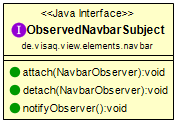
\includegraphics[scale = 0.6]{media/frontend/view/de.view.elements.navbar/ObservedNavbarSubjectClass.png}
    \end{figure}
    \end{minipage} \hfill
\begin{minipage}{0.6\textwidth}
Ein Interface für das von dem NavbarObserver beobachtete Subjekt, welches den Observer über Änderungen informiert.  Es handelt sich hierbei um ein Element aus dem Beobachter Entwurfsmuster.
\end{minipage}

Methoden:
\begin{itemize} 
    \item \emph{public void attach(NavbarObserver navbarObserver)} Erstellt eine Verbindung aus der Liste der Observer, zwischen dem Observer und Subjekt her
    \item \emph{public void detach(NavbarObserver navbarObserver)} Entfernt die Verbindung aus der Liste der Observer, zwischen dem Observer und Subjekt
    \item \emph{public void notifyObserver()} Informiert den Observer über Änderungen
\end{itemize}


\rule{\textwidth}{0.4pt} 
\class{Timeline}
public class Timeline implements NavbarElement

\begin{minipage}{0.3\textwidth}
    \begin{figure}[H]
        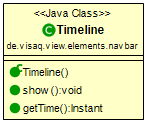
\includegraphics[scale = 0.7]{media/frontend/view/de.view.elements.navbar/TimelineClass.png}
    \end{figure}
    \end{minipage} \hfill
\begin{minipage}{0.6\textwidth}
Die Timeline ist ein Regulator welcher aufgerufen werden kann und die historischen Daten direkt auf der Karte darstellt. Es implementiert außerdem NavbarElement um die dazugehörige show Methode zu verwenden.
\end{minipage}

Methoden:
\begin{itemize} 
    \item \emph{public void show()} Zeigt die historischen Daten mithilfe eines Regulators an 
    \item \emph{public void getTime()} Gibt das aktuelle Zeitfenster, welches von dem Regulator ausgewählt wurde zurück
\end{itemize}

\rule{\textwidth}{0.4pt} 
\class{Toolbar}
public class Toolbar implements NavbarElement

\begin{minipage}{0.3\textwidth}
    \begin{figure}[H]
        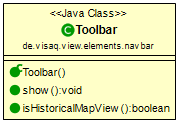
\includegraphics[scale = 0.6]{media/frontend/view/de.view.elements.navbar/ToolbarClass.png}
    \end{figure}
    \end{minipage} \hfill
    \begin{minipage}{0.6\textwidth}
Zeigt dem Benutzer die einzelnen Links und Beschreibungen zu den einzelnen Funktionen
\end{minipage}

Methoden:
\begin{itemize} 
    \item \emph{public Toolbar()} Konstruktor für die Toolbar
    \item \emph{public void show()} Zeigt die Toolbar
    \item \emph{public boolean isHistoricalMapView()} Gibt zurück ob die historicalMapView aktiviert wurde oder nicht
    \item \emph{private void setHistoricalMapView(boolean historicalMapView)} Aktiviert die historicalMapView
\end{itemize}

\rule{\textwidth}{0.4pt} 
\class{NavbarElement}
public interface NavbarElement 

\begin{minipage}{0.3\textwidth}
    \begin{figure}[H]
        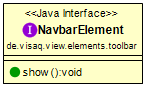
\includegraphics[scale = 0.7]{media/frontend/view/de.view.elements.navbar/NavbarElementClass.png}
    \end{figure}
\end{minipage} \hfill
\begin{minipage}{0.6\textwidth}
Interface für alle Elemente welche in der Navbar gezeigt werden können. 
\end{minipage}

Methoden:
\begin{itemize} 
    \item \emph{public void show()} Zeigt die einzelnen Elemente auf der Schnittstelle
\end{itemize}
